\documentclass[border=10pt]{standalone}
\usepackage{tikz}
\usepackage{xcolor}

% Cargar bibliotecas adicionales de TikZ
\usetikzlibrary{shapes.geometric} % Biblioteca para formas geométricas como cilindros
\usetikzlibrary{calc}
\usetikzlibrary{decorations.markings}
\usetikzlibrary{shadows.blur}
\usetikzlibrary{fadings}

\begin{document}

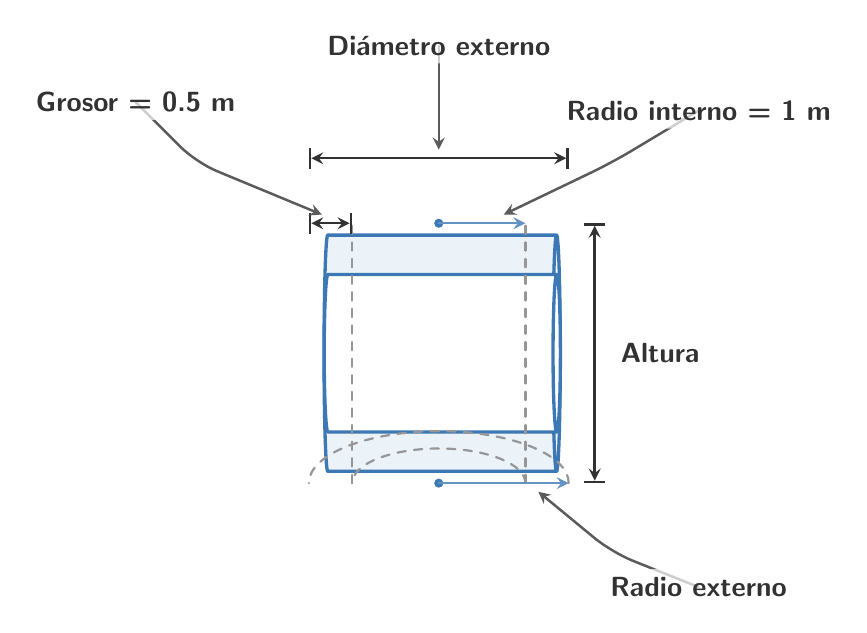
\begin{tikzpicture}[
  % Definir estilos globales para mejorar la apariencia
  line cap=round,
  line join=round,
  >=stealth, % Flechas más elegantes
  thick, % Líneas más gruesas por defecto
  scale=1.1, % Escalar ligeramente toda la figura
]

% Definimos algunas variables utilizando \pgfmathsetmacro
\pgfmathsetmacro{\altura}{3} % Altura del cilindro (unidad arbitraria, ej: metros)
\pgfmathsetmacro{\radiointerno}{1} % Radio interno
\pgfmathsetmacro{\grosor}{0.5} % Grosor de la pared
\pgfmathsetmacro{\radioexterno}{\radiointerno + \grosor} % Radio externo = 1 + 0.5 = 1.5

% Definir proporciones para la perspectiva
\pgfmathsetmacro{\proporcionY}{0.4} % Proporción para la perspectiva vertical

% Definir colores personalizados
\definecolor{cilindroColor}{RGB}{60, 120, 180} % Azul para el cilindro
\definecolor{lineaOculta}{RGB}{150, 150, 150} % Gris para líneas ocultas
\definecolor{etiquetaColor}{RGB}{50, 50, 50} % Gris oscuro para etiquetas

% Coordenadas de los centros de las bases
\coordinate (centroinferior) at (0,0);
\coordinate (centrosuperior) at (0,\altura);

% Definir puntos clave para las mediciones
% Base inferior
\coordinate (R0b) at (\radioexterno, 0); % Punto derecho externo inferior
\coordinate (-R0b) at (-\radioexterno, 0); % Punto izquierdo externo inferior
\coordinate (r0b) at (\radiointerno, 0); % Punto derecho interno inferior
\coordinate (-r0b) at (-\radiointerno, 0); % Punto izquierdo interno inferior
% Base superior
\coordinate (R0t) at (\radioexterno, \altura); % Punto derecho externo superior
\coordinate (-R0t) at (-\radioexterno, \altura); % Punto izquierdo externo superior
\coordinate (r0t) at (\radiointerno, \altura); % Punto derecho interno superior
\coordinate (-r0t) at (-\radiointerno, \altura); % Punto izquierdo interno superior

% --- Dibujo del cilindro externo usando shapes.geometric ---
\node[cylinder,
      draw=cilindroColor,
      line width=1.2pt,
      aspect=\proporcionY,
      minimum height=\altura cm,
      minimum width=2*\radioexterno cm,
      anchor=center,
      cylinder uses custom fill,
      cylinder body fill=cilindroColor!10,
      cylinder end fill=cilindroColor!5]
      (cilindroExterno) at (0, \altura/2) {};

% --- Dibujo del cilindro interno (hueco) usando shapes.geometric ---
\node[cylinder,
      draw=cilindroColor,
      line width=1.2pt,
      aspect=\proporcionY,
      minimum height=\altura cm,
      minimum width=2*\radiointerno cm,
      anchor=center,
      cylinder uses custom fill,
      cylinder body fill=white,
      cylinder end fill=white]
      (cilindroInterno) at (0, \altura/2) {};

% Añadir líneas adicionales para mejorar la visualización 3D
% Arcos traseros (ocultos) para dar sensación de profundidad
\draw[dashed, lineaOculta, line width=0.8pt] (R0b) arc (0:180:{\radioexterno} and {\proporcionY*\radioexterno});
\draw[dashed, lineaOculta, line width=0.8pt] (r0b) arc (0:180:{\radiointerno} and {\proporcionY*\radiointerno});

% Añadir líneas ocultas (dashed) para mejorar la visualización
\draw[dashed, lineaOculta, line width=0.8pt] (-r0b) -- (-r0t);
\draw[dashed, lineaOculta, line width=0.8pt] (r0b) -- (r0t);

% Puntos centrales (opcionales)
\fill[cilindroColor] (centroinferior) circle (1.5pt);
\fill[cilindroColor] (centrosuperior) circle (1.5pt);

% --- Dimensiones y etiquetas ---
% Definir estilos para etiquetas y líneas de medición
\tikzset{
  etiqueta/.style={font=\sffamily\bfseries, text=etiquetaColor, align=center},
  linea_medicion/.style={|<->|, line width=0.9pt, color=etiquetaColor},
  linea_indicadora/.style={->, rounded corners=8pt, line width=0.9pt, color=etiquetaColor!80},
  linea_radio/.style={->, line width=0.9pt, color=cilindroColor!80}
}

% Altura (colocar etiqueta directamente junto al segmento)
\coordinate (alturaInicio) at ($(R0b) + (0.3, 0)$);
\coordinate (alturaFin) at ($(R0t) + (0.3, 0)$);
\draw [linea_medicion] (alturaInicio) -- (alturaFin);
\node[etiqueta, right=0.2cm] at ($(alturaInicio)!0.5!(alturaFin)$) {Altura};

% Radio interno = 1 m (mantener línea original y añadir etiqueta alejada)
\draw [linea_radio] (centrosuperior) -- (r0t);
\coordinate (etiquetaRadioInterno) at ($(centrosuperior) + (3.0, 1.3)$);
\coordinate (puntoControlRadioInterno) at ($(etiquetaRadioInterno) + (-1.0, -0.6)$);
\coordinate (puntoFinalRadioInterno) at ($(centrosuperior)!0.65!(r0t) + (0.1, 0.1)$);
\draw [linea_indicadora] (etiquetaRadioInterno) -- (puntoControlRadioInterno) -- (puntoFinalRadioInterno);
\node[etiqueta, fill=white, fill opacity=0.7, text opacity=1, rounded corners=3pt, inner sep=3pt] at (etiquetaRadioInterno) {Radio interno = \radiointerno{} m};

% Grosor = 0,5 m (mantener línea original y añadir etiqueta alejada) - Movido a la izquierda
\draw [linea_medicion] (-r0t) -- (-R0t);
\coordinate (etiquetaGrosor) at ($(-R0t) + (-2.0, 1.4)$);
\coordinate (puntoControlGrosor) at ($(etiquetaGrosor) + (0.7, -0.7)$);
\coordinate (puntoFinalGrosor) at ($(-r0t)!0.5!(-R0t) + (-0.1, 0.1)$);
\draw [linea_indicadora] (etiquetaGrosor) -- (puntoControlGrosor) -- (puntoFinalGrosor);
\node[etiqueta, fill=white, fill opacity=0.7, text opacity=1, rounded corners=3pt, inner sep=3pt] at (etiquetaGrosor) {Grosor = \grosor{} m};

% Diámetro externo (mantener línea original y añadir etiqueta alejada)
\coordinate (diamExtIzq) at ($(-R0t) + (0, 0.75)$);
\coordinate (diamExtDer) at ($(R0t) + (0, 0.75)$);
\draw [linea_medicion] (diamExtIzq) -- (diamExtDer);
\coordinate (etiquetaDiametro) at ($(diamExtIzq)!0.5!(diamExtDer) + (0, 1.3)$);
\coordinate (puntoControlDiametro) at ($(etiquetaDiametro) + (0, -0.6)$);
\coordinate (puntoFinalDiametro) at ($(diamExtIzq)!0.5!(diamExtDer) + (0, 0.1)$);
\draw [linea_indicadora] (etiquetaDiametro) -- (puntoControlDiametro) -- (puntoFinalDiametro);
\node[etiqueta, fill=white, fill opacity=0.7, text opacity=1, rounded corners=3pt, inner sep=3pt] at (etiquetaDiametro) {Diámetro externo};

% Radio externo (mantener línea original y añadir etiqueta alejada)
\draw [linea_radio] (centroinferior) -- (R0b);
\coordinate (etiquetaRadioExterno) at ($(centroinferior) + (3.0, -1.2)$);
\coordinate (puntoControlRadioExterno) at ($(etiquetaRadioExterno) + (-1.0, 0.4)$);
\coordinate (puntoFinalRadioExterno) at ($(centroinferior)!0.7!(R0b) + (0.1, -0.1)$);
\draw [linea_indicadora] (etiquetaRadioExterno) -- (puntoControlRadioExterno) -- (puntoFinalRadioExterno);
\node[etiqueta, fill=white, fill opacity=0.7, text opacity=1, rounded corners=3pt, inner sep=3pt] at (etiquetaRadioExterno) {Radio externo};

\end{tikzpicture}

\end{document}
